% vim: textwidth=78 ai spell spelllang=en
\documentclass[conference]{IEEEtran}
\usepackage[utf8]{inputenc}
\usepackage[IL2]{fontenc}
\usepackage{graphicx}
\usepackage{url}
\usepackage{subfig}
\usepackage{xspace}

%\documentclass[a4paper]{easychair}

% In order to save space or manage large tables or figures in a
% landcape-like text, you can use the rotating and pdflscape
% packages. Uncomment the desired from the below.
%
% \usepackage{rotating}
% \usepackage{pdflscape}

\usepackage{color}
\newcommand\Color[2]{\textcolor{#1}{#2}}
\newcommand{\nb}[1]{\marginpar{\scriptsize #1}}
%\newcommand\todo[1]{\nb{\Color{red}{#1}}}
%\renewcommand\todo[1]{}

\newcommand\tp{\textsc{TakePlace}\xspace}

\begin{document}

\title{Web-based Service for Collaborative Organization of Academic Events --
Case Study of "TakePlace"}

\author{\IEEEauthorblockN{Jaroslav \v{S}krab\'{a}lek}
\IEEEauthorblockA{Faculty of Informatics\\
Masaryk University\\
Brno, Czech Republic\\
Email: xskraba1@fi.muni.cz}
\and
\IEEEauthorblockN{Tom\'{a}\v{s} Lud\'{i}k}
\IEEEauthorblockA{Faculty of Informatics\\
Masaryk University\\
Brno, Czech Republic\\
Email: xludik2@fi.muni.cz}
\and
\IEEEauthorblockN{Ji\v{r}\'{i} Slab\'{y}}
\IEEEauthorblockA{Faculty of Informatics\\
Masaryk University\\
Brno, Czech Republic\\
Email: xslaby@fi.muni.cz}
\and
\IEEEauthorblockN{Tom\'{a}\v{s} Pitner}
\IEEEauthorblockA{Faculty of Informatics\\
Masaryk University\\
Brno, Czech Republic\\
Email: tomp@fi.muni.cz}}

\sloppy
\maketitle

\begin{abstract}
The changes that the "Web 2.0" brings into the development of rich internet
applications and online project management are taken into account in this
paper. Namely development of a web-based service \tp, a case study
project aimed at online event management, is described. The service deals with
planning, managing and promoting professional events. The paper characterizes
its functionality analysis and design, presents methods of realization and
outlines the expected impact on building professionally-oriented online social
communities.
\end{abstract}

\section{Introduction}
The Internet from the Web 2.0 point of view is not only a provider of static,
passive information, but also a provider of functionality to its end
users. Thus the Internet became a \emph{standalone platform} offering
\emph{Rich Internet Applications} (RIA) -- modern web-based services
\cite{o2007web}. Increasing complexity and usability of RIA has changed
people's understanding of the Internet. Thanks to the web technology
advancements, companies started a transition from desktop services to the
Internet. During this period, processes of the web transformation have been
replaced in favor of the higher level of Internet development.

Besides the meaning of Web 2.0 and what it means for the Internet, ICT and
society, there are significant questions regarding the software development
\cite{pitner-priklady}. We can date the first bases of a systematic project
management to the beginning of the 20th century.

Since then many approaches
and software development processes have been established and introduced into
the practice \cite{stellman2005applied}. From simple models like the Waterfall
we went through Critical Chain Project Management, Extreme Project Management
including Scrum and Agile Software Development to the sophisticated
methodologies like PRINCE2 or Rational Unified Process by IBM. But those
approaches result from an earlier degree of software development appropriate
to desktop programs.

Web 2.0 projects have significant differences such as:
\begin{itemize}
\item development stage of \textbf{"perpetual beta"},
\item \textbf{rapid deployment} or absence of software release cycle,
\item \textbf{lightweight} programming \textbf{models},
\item dynamic \textbf{scalability},
\item \textbf{sampling} and \textbf{testing},
\item \textbf{sharing} the web-based services with many users,
\item ability of \textbf{collaborative work} and
\item \textbf{accessing the data wherever} the users are.
\end{itemize}

On the contrary, desktop programs are primarily used by one user, on one
computer (or small local network) using local computer (local network)
resources. The differences mentioned above require special approaches being
distinguished from the classical ones \cite{o2007web}. Therefore there is a
need for project management approach combining such classical methodologies
with more complex approaches while reflecting the necessity of proper business
models closely connected to the development, efficiency and performance of
RIA, security issues, etc. \cite{vossen2007unleashing}.

This modern approach shall not only focus on the development itself but,
according to contemporary trends of humanistic approaches, to the developers
who back up every single project and the project's success depends much on
them \cite{motschnig2002learning}.

\section{Motivation from Practice}
We developed an information system and web-based service \tp
(depicted in Fig.~\ref{fig-takeplace} for illustration). It is a system for
efficient and transparent organization and management of professional events
(conferences, symposia, congresses, seminars, etc.).  During the development
phase, we have tested some \emph{new ways of IT project management}
\cite{user-centered2010} enriched by the \emph{Person-Centred
Approach}\footnote{Person-Centered Approach was introduced by the American
psychologist Carl Rogers. The essentials are three attitudinal conditions
according to Rogers, which they are motive power in personal development of
each person. These conditions are: acceptance (unconditional positive regard),
emphatic understanding and congruence.  Congruence expresses personal
integrity composing from experiences and feelings in mutual complementation.
Integrity comprises acceptance and emphatic understanding as well. Those
attitudes are beneficial for all relationships characterized by psychical
development -- relationship between child and parents, partners, or
relationship between manager and developer too.} (PCA) principles
\cite{derntl2004r}. Development of modern web-based services and more generally
the whole Web 2.0 environment is very appropriate for application in new
\emph{humanistic management approaches} with outlook emphasizing common human
needs. It should build up a unity to achieve the community of persons
to become stronger as a community \cite{mele2003challenge}.  In addition,
thanks to changes of understanding the Internet by people using Web 2.0
services -- RIA -- new researching methodology adapts current complex
approaches from development processes to management right for the Internet
environment.

Our motivation was and still is to provide, from an operating point of view,
simple yet functionally rich tools with a high utility value for organizers of
academic events. The goal is to \emph{address the professional public} and
\emph{build a professional community} of academic and expert users,
\emph{sharing their know-how} with others in the spirit of the current
trends of modern web-based services.  The \tp shields the creation of a
wide range of professional communities. Based on professional outcome, sharing
a new social portal will arise providing information and associational
functions including knowledge library of conference papers, posters and other
artefacts.

In order to choose proper Web 2.0 tools, special visual patterns and
specifications of PCA are implemented during the development of \tp
service. Both parts of the web system -- user and administrative -- are
considered and the need of usability and support is discussed. The \tp
system demonstrates implementation principles of user-centeredness and
process-orientation.

\section{Academic Conference -- Case Study}
The \tp product is a \emph{web-based service} designed and implemented
on the basis of expert requirements for the appropriate tool to facilitate
\emph{efficient organization of events} based on meeting, sharing and
communication. \tp covers a wide range of sophisticated organizational
processes with unified user interface. The system combines a number of
software products -- an email client, word processor, database of contacts,
accounting module for budget registration of the event, payment portal, etc.

The user is provided with a web interface and gains an access to the standard
services for organizing events according to the type. Basic types of events
include conferences, congresses, symposia, seminars, trainings, consultation
meetings, workshops and team buildings. \tp differs from its competitors by a
unique set of features.

In addition to the advanced organizational system, it offers its users
advanced services like a tool for creating web presentations based on
interactive professional templates developed by experienced graphic designers,
historical continuity of given events, uniform terminology in the context of
professional event series, the payment portal, easy creation of promotional
materials and elements of the visual information system, assembling and
typesetting proceedings and much more. The great advantage is the overall
reduction in costs for the management and organization of professional events
and saving thus resources otherwise needed for graphic design or spent on
software equipment for instance.

\begin{figure*}[tb]
\begin{centering}
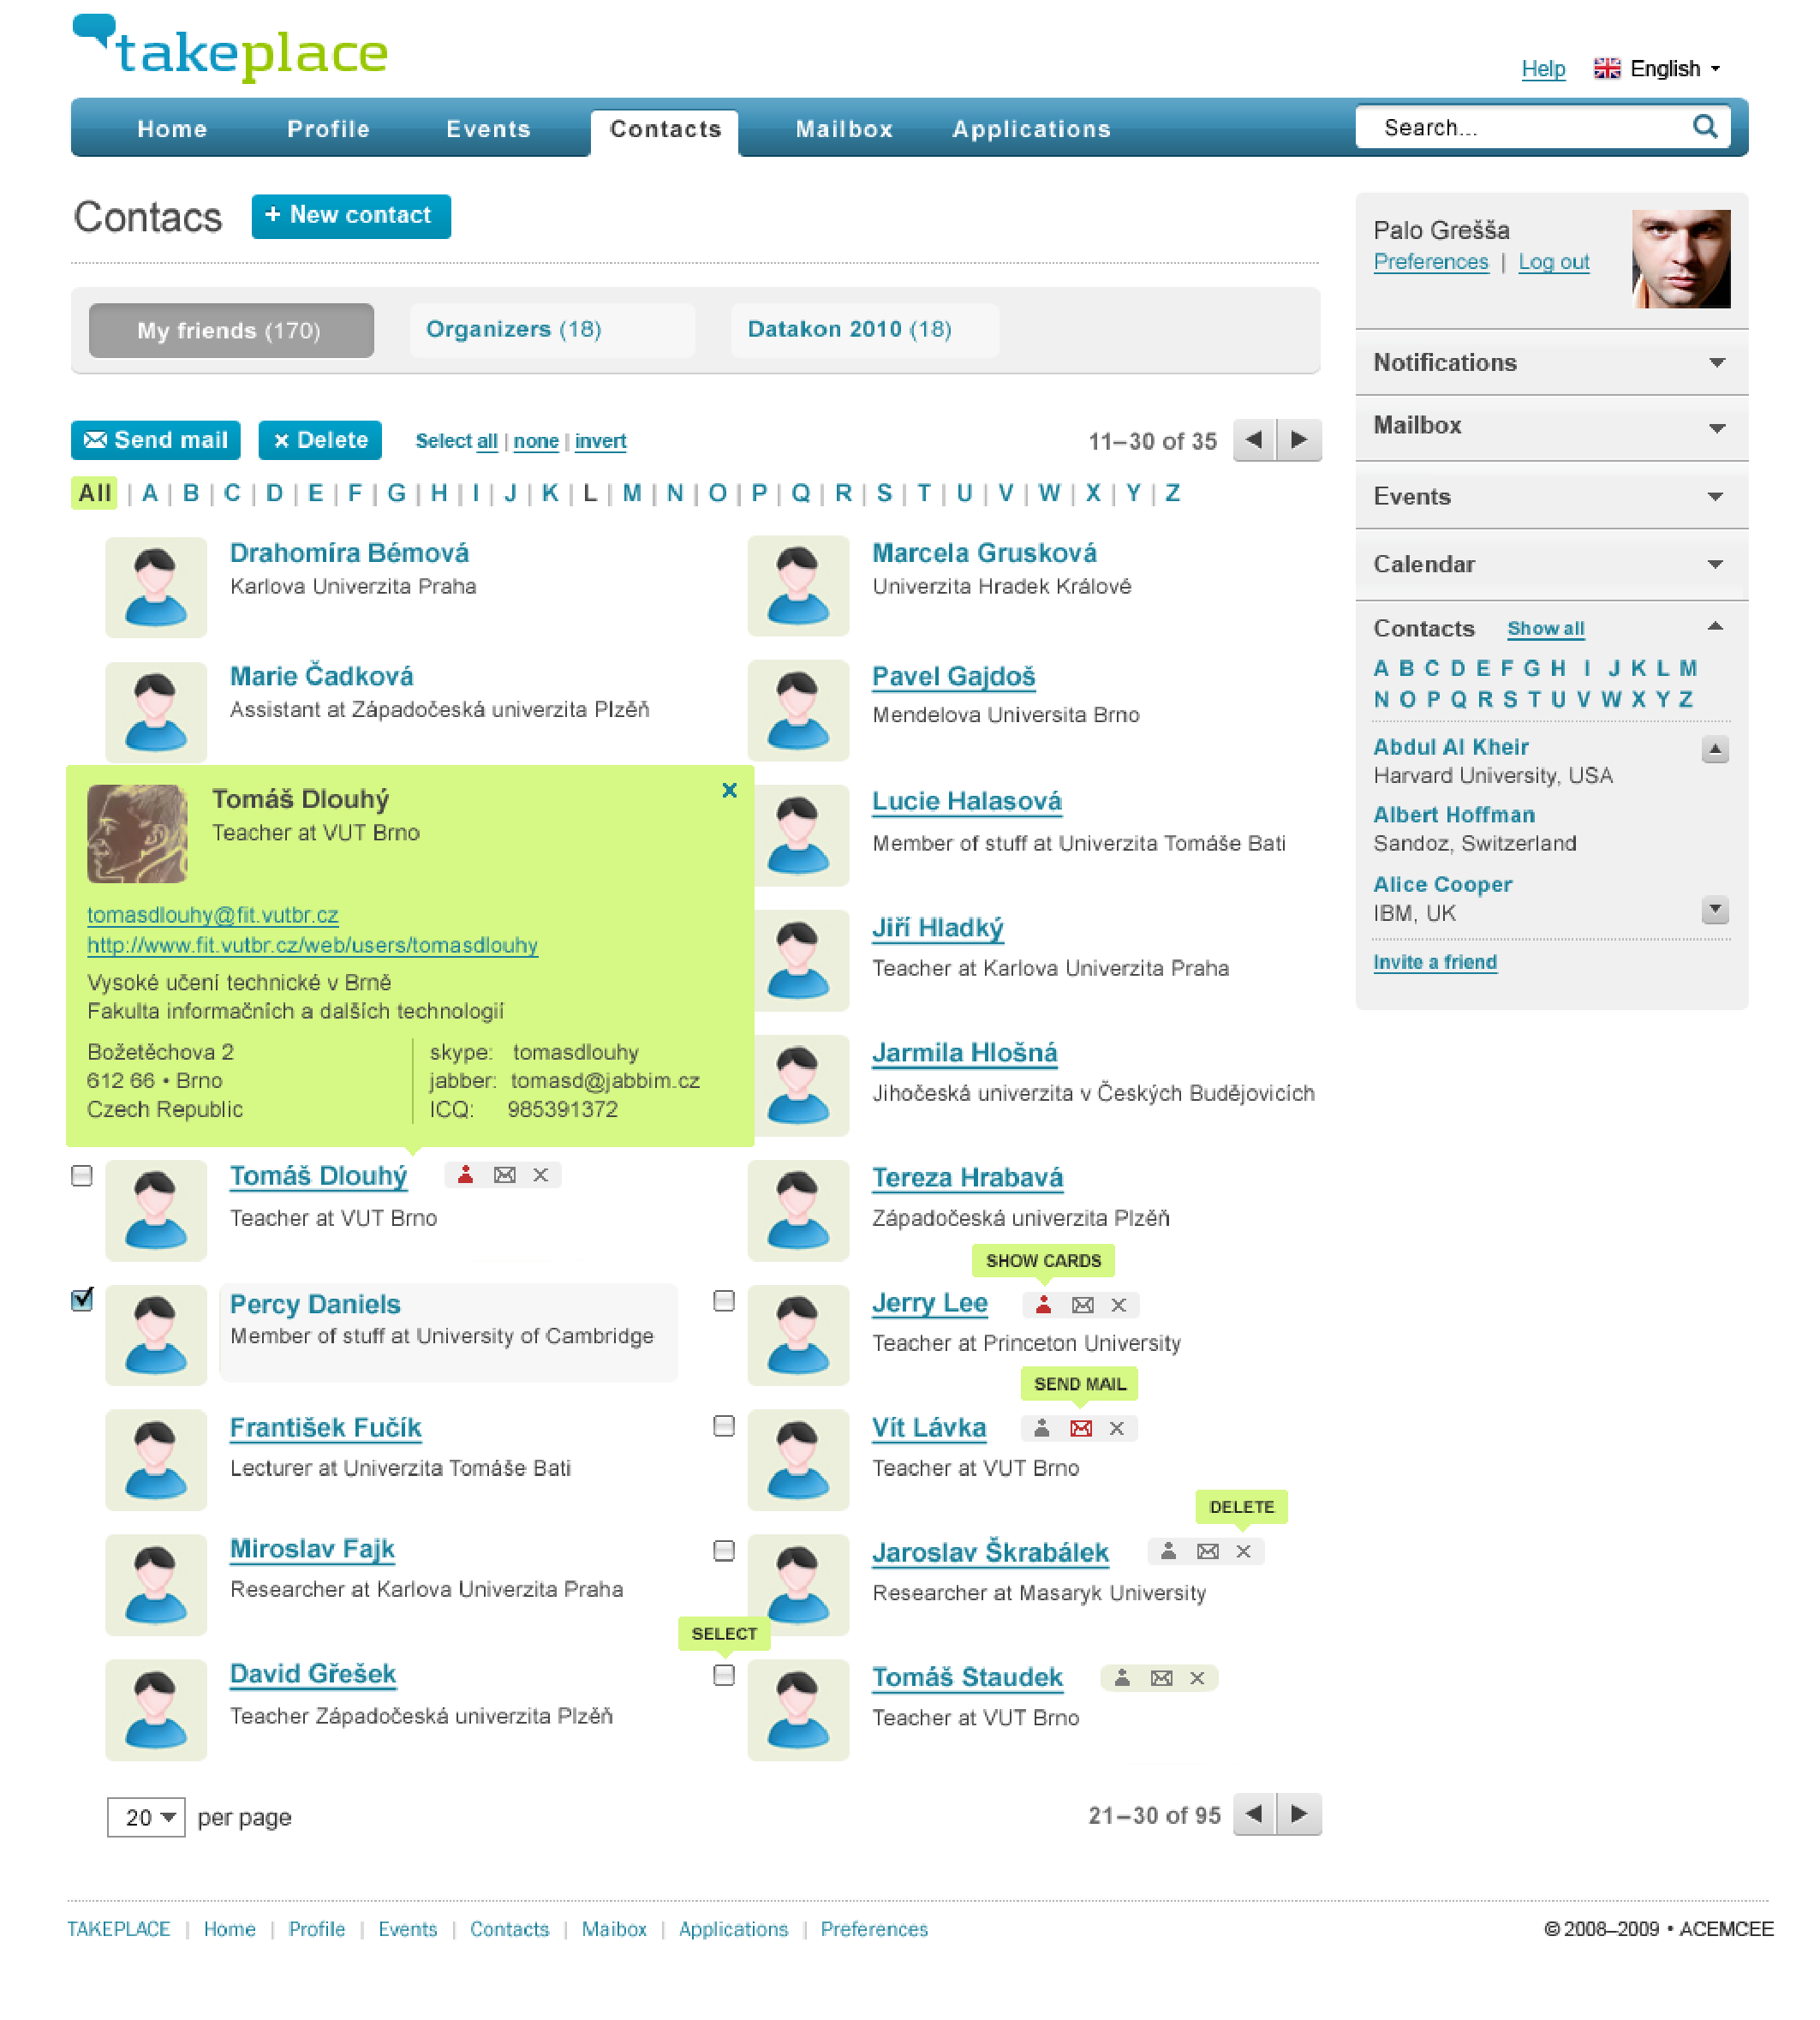
\includegraphics[width=0.8\textwidth]{tp-contacts}
\caption{\tp -- Contacts}
\label{fig-takeplace}
\end{centering}
\end{figure*}

The \tp system is characterized by advanced \emph{awareness} (alert subsystem)
of various aspects of the event -- approaching deadlines, not receiving
outputs from involved people, exceeding quotas, etc. Thus the entire
administrative organization is considerably easy. The \emph{uniform
terminology} is reached due to the historical continuity and coherence in case
of annual series of events.  All events held within the system are
\emph{archived} and \emph{available} for visitors forever (unless they are
removed by the event owner). In addition to the organizational system, \tp
offers a user-friendly website creation and printing materials with
professional graphics. The system is characterized by simple and intuitive
graphical user interface, even though a rich set of diverse functions is
offered.

Academic institutions are mainly oriented to professional training events of
greater magnitude and importance \cite{pitner2007person}. They appreciate
applications that are easy to use and have intuitive interface, but lay
emphasis on the advanced features with formal presentation. In addition to
these functions there are modules for creating proceedings, review functions,
advanced programming, creation of specific meetings among visitors and
special presentation styles. To the motivation mentioned earlier we can also
add the cooperation of organizational teams and professional output presented
here.

A \emph{practical example} of an event organization may be outlined on a part
of the process of organizing a professional conference:
\begin{enumerate}
\item The chief organizer assigns involved colleagues in the organizing and
program committees and assigns them roles such as evaluator, assistant, etc. 
\item The program committee together with organizers determines milestones --
important dates and terms. 
\item Potential speakers are then approached with an offer of contributed
presentation. 
\item They upload their submission on a server via the web interface. 
\item The submission will be assigned to a particular evaluator by the program
committee. 
\item According to the review criteria, one or several evaluations are done. 
\item The members of committee compile the professional program from
contributions meeting the conference requirements. Aspects such as possible
inclusion of the same speaker to more lectures at the same time, or the
selection of lectures which cannot be realized at the same time are taken into
consideration when creating the program. The program can be designed in a
linear form of timeline, conceivably it is possible to extend the program into
more sections (horizontal concept) or blocks (vertical concept).
\end{enumerate}

The attractiveness increases the number of links pointing to the web and
web-based services and catalyze creating of appropriate professional users'
communities. With increasing number of professional events organized with the
\tp system, it will be able to create an \emph{evaluation} of these events.
Users will be able to share the experience of participation, evaluate and
recommend events to others. Virtual communities of professional users arise in
course of time.  The emphasis on social and interpersonal interaction is
essential feature of \tp.

\section{Web-based Service Development}
The \tp system is built upon a robust technology \emph{Java 2 Enterprise
Edition} (J2EE) integrating number of free frameworks. These solutions are used
mainly in the fields requiring stability, security, flexibility and
manageability \cite{racek2006is}. The \tp service is a platform
consisting of several modules (Registration, Conference Administration,
Submission, Schedule, Accommodation, Transportation and Content Management
System). Each module represents an added value to the whole system, to each
event with various characters.

\subsection{Analysis}
Our main objective is to design well a web-based system for collaborative
organization of academic conferences. That is the reason why analysis is the
key phase \cite{kubicek-emergency}. The developed system is large-scaled so we
focused in the paper primarily on \emph{Registration} and \emph{Conference
Administration} modules. The analysis consists of two basic levels. The
functional view is represented by \emph{Use Case Diagram}
(Fig.~\ref{fig-usecase}) and the data view is represented by \emph{Entity
Relation Diagram} (Fig.~\ref{fig-erd}).

\begin{figure*}[tb]
\begin{centering}
\subfloat[Use Case
Diagram]{\label{fig-usecase}
\includegraphics[width=0.5\textwidth]{usecase}}
\subfloat[Logical Data
Model]{\label{fig-erd}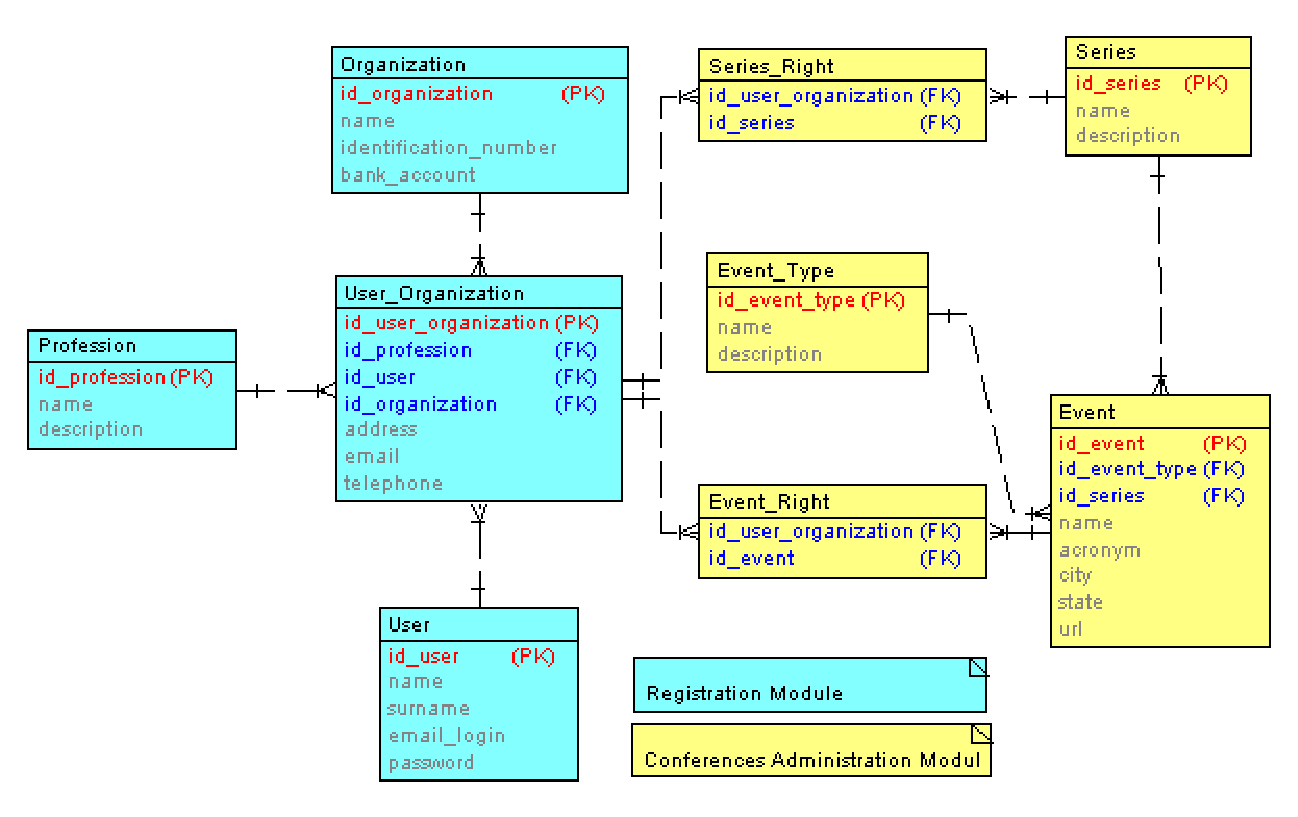
\includegraphics[width=0.5\textwidth]{erd}}
\caption{\tp models}
\end{centering}
\end{figure*}

The use case diagram describes the functionality for Anonymous users, who can
\emph{Register} or \emph{Log-in} to the web-based system. The third (and last)
function for anonymous user is sending a new password in case of the old one
is lost.  The registered \emph{User} can edit personal details and, in case
they work in several organisations, also the information about their
affiliation.  The user can find appropriate event or series based on searching
criteria. The \emph{Event Owner} comprehends a functionality to register an
event and eventually edit it. Next use case represents setting the user rights
for the event. The \emph{Series Owner} has the same functionality as
\emph{Event Owner}, but instead of events the user administrates series.

Entity relation diagram represents the data view on the web-based application.
The entities \emph{User}, \emph{User\_Organisation} and \emph{Organisation}
store personal information about the user and user's organisation. The system
offers large scalability for the user. A user can insert more organisations
where they are working and for every organization set up a profession selected
from code list.

The second part of the data model describes \emph{Event} and \emph{Series}
administration. \tp allows the user assigning events to the series and
granting user rights to the specific series or events. Events can also be
classified by types. In Fig.~\ref{fig-erd} there is depicted the logical data
model for better understanding.

\subsection{Design}
Standard three-layer architecture is a basis of \emph{three large frameworks}
used in the system.

Presentation layer is realized by \emph{Google Web Toolkit 2.0}
(GWT)\footnote{All information about GWT are at
\url{http://code.google.com/intl/cs/webtoolkit/}}, which
offers tools for creating complex, object-oriented graphical user interfaces
based upon \emph{Asynchronous JavaScript and XML} (AJAX) techniques. Thanks to
this, a rich user experience is provided and the \tp service becomes truly Web
2.0 application with all benefits.

Business layer uses popular and very sophisticated solution \emph{Spring
Framework}\footnote{Detailed description with packages to download available at
\url{http://www.springsource.org/}.}. Thanks to this framework, performance and reliability as well as
flexibility of the whole system are ensured. It is very important mainly in
distributed environment for which \tp is primarily designed.

In the end, persistent layer uses the well-known J2EE applications'
object-relation mapping \emph{Hibernate}. It helps \tp to maintain pure
principles of object-oriented development. Hibernate works upon
\textsc{PostgreSQL} as a Database Management System (DBMS).
\textsc{PostgreSQL} is one of the most powerful open-source database systems
in the world with the wide support of SQL standards (92, 99, 2003,
\ldots)\footnote{See \url{http://www.postgresql.org/} for more technical
documentation.}.

\subsection{Realization}
Architecture of the \tp service is realized with the \emph{Star
topology}.
Administrative application serves as the central node. It is responsible for
event and user management. Individual administrative nodes represent
independent applications placed world-wide on different servers. Events are
assigned to servers according to their geo-location. Each so-called
\emph{Overseer} node administers events in a separate database space, which
results in stronger data security.

\subsection{Current Development State}
The \tp service is currently in the stage of testing and finishing its
first functional unit that will be offered publicly during summer 2010.
Till now the first stage of \tp development (beta) is running in pilot where
specifically chosen users are using \tp for academic conference organization.
This helps us very much in the system adaptation according to users' needs.

The service is being presented at \url{http://www.takeplace.eu/} along with
feature description, user feedback and video tour.

\section{Conclusions -- Future Work}
In the next six months we plan to finish the implementation of the main
functionality of academic conference workflow and aim to the second workflow,
namely seminars and workshops.

Our main objective is to design a \emph{modular web-based system for
collaborative organization of professional events}. The core modules of the
system are Registration, Submission, Schedule, Accommodation, Transportation,
Content Management and Conference Administration. The system being developed
is large-scaled; in the paper we focused primarily on the Registration and
Conference Administration modules. Developing the remaining modules is our
plan for the near future.

The long-term goal is then to establish a \emph{professional community} of
authors who communicate in virtual communities and share their knowledge via
the online \emph{knowledge base}.

\section*{Acknowledgements}
The contribution is a part of the Project (No. 2615/2010/G1) called "New
Approaches to the Software Development Education" and Research Plan
(MSM0021622418) called "Dynamic Geovisualization in Crisis Management", both
of them supported by the Ministry of Education, Youth and Sports, Czech
Republic.

\newpage

\bibliographystyle{plain} 
\bibliography{woss2010}

\end{document}
